% Chapter 3: Protocol Architecture
\chapter{Protocol Architecture}
\label{ch:architecture}

This chapter presents the high-level architecture of the \tprotocol{} protocol, describing the roles of each component, the flow of payment information through the system, and the trust model that ensures secure operation.

\section{Architectural Principles}
\label{sec:arch-principles}

The \tprotocol{} protocol is built on three fundamental architectural principles:

\begin{enumerate}
    \item \textbf{Separation of Concerns}: Payment logic, transport encoding, and blockchain operations are cleanly separated into independent layers.

    \item \textbf{Trust Minimization}: No single party can unilaterally redirect funds or forge payments. The blockchain serves as the ultimate source of truth.

    \item \textbf{Extensibility}: New payment schemes, transport layers, and blockchain networks can be added without modifying core protocol components.
\end{enumerate}

\section{System Components}
\label{sec:components}

The \tprotocol{} protocol involves three primary actors, each with distinct responsibilities and trust boundaries.

\begin{figure}[ht]
\centering
\resizebox{\textwidth}{!}{%
\begin{tikzpicture}[
    node distance=1.8cm and 2.2cm,
    component/.style={
        rectangle,
        rounded corners=6pt,
        minimum width=2.8cm,
        minimum height=1.6cm,
        line width=1.5pt,
        font=\bfseries
    },
    subcomponent/.style={
        rectangle,
        rounded corners=3pt,
        minimum width=2.2cm,
        minimum height=0.5cm,
        font=\footnotesize
    },
    blockchain/.style={
        rectangle,
        rounded corners=6pt,
        minimum width=9cm,
        minimum height=1.2cm,
        draw=orange,
        line width=2pt,
        fill=orange!10,
        font=\bfseries
    },
    arrow/.style={->, >=stealth, line width=1.2pt, violet},
    label/.style={font=\scriptsize, fill=white, inner sep=1pt}
]

% Main components
\node[component, draw=blue, fill=blue!10] (client) {Client};
\node[component, draw=violet, fill=violet!10, right=of client] (server) {Server};
\node[component, draw=green!60!black, fill=green!10, right=of server] (facilitator) {Facilitator};

% Subcomponents
\node[subcomponent, draw=blue, fill=blue!5, below=0.2cm of client.south] (wallet) {Wallet};
\node[subcomponent, draw=violet, fill=violet!5, below=0.2cm of server.south] (middleware) {Middleware};
\node[subcomponent, draw=green!60!black, fill=green!5, below=0.2cm of facilitator.south] (settler) {Settler};

% Blockchain layer
\node[blockchain, below=2.5cm of server] (blockchain) {Blockchain};

% Blockchain sub-elements
\node[subcomponent, draw=orange, fill=orange!5] at ([xshift=-2.5cm]blockchain.center) (evm) {EVM};
\node[subcomponent, draw=orange, fill=orange!5] at ([xshift=-0.8cm]blockchain.center) (solana) {Solana};
\node[subcomponent, draw=orange, fill=orange!5] at ([xshift=0.8cm]blockchain.center) (ton) {TON};
\node[subcomponent, draw=orange, fill=orange!5] at ([xshift=2.5cm]blockchain.center) (tron) {TRON};

% Arrows with labels
\draw[arrow] (client) -- node[label, above] {1. Request} (server);
\draw[arrow, bend right=20] (server.south west) to node[label, below] {2. 402} (client.south east);
\draw[arrow, bend right=20] (client.north east) to node[label, above] {3. Pay} (server.north west);
\draw[arrow] (server) -- node[label, above] {4. Verify} (facilitator);
\draw[arrow] (facilitator.south) -- node[label, right] {5. Settle} (blockchain.east);

\end{tikzpicture}%
}
\caption{T402 System Architecture}
\label{fig:architecture}
\end{figure}

\subsection{Client}
\label{subsec:client}

The \term{Client} is any application or agent that requests access to protected resources. Clients are responsible for:

\begin{itemize}
    \item \textbf{Wallet Management}: Maintaining private keys securely and signing payment authorizations
    \item \textbf{Payment Construction}: Creating properly formatted \code{PaymentPayload} structures
    \item \textbf{Scheme Selection}: Choosing from available payment options in the \code{accepts} array
    \item \textbf{Error Handling}: Responding appropriately to payment failures and retrying when appropriate
\end{itemize}

Clients may take various forms:

\begin{table}[h]
\centering
\caption{Client Types and Characteristics}
\label{tab:client-types}
\begin{tabular}{llp{5cm}}
\toprule
\textbf{Type} & \textbf{Signing} & \textbf{Use Case} \\
\midrule
Browser App & Wallet extension & Interactive web payments \\
Backend Service & Programmatic key & Automated API access \\
AI Agent & MCP integration & Autonomous resource acquisition \\
CLI Tool & Local keystore & Developer testing \\
Mobile App & Secure enclave & Consumer applications \\
\bottomrule
\end{tabular}
\end{table}

\subsection{Resource Server}
\label{subsec:resource-server}

The \term{Resource Server} provides access to protected resources---APIs, content, data, or computational services---and defines the payment requirements for access.

\textbf{Responsibilities}:

\begin{enumerate}
    \item \textbf{Requirement Definition}: Specify acceptable payment methods including:
    \begin{itemize}
        \item Payment scheme (e.g., ``exact'')
        \item Supported networks (e.g., \code{eip155:8453})
        \item Required amount in atomic units
        \item Token contract address
        \item Recipient wallet address (\code{payTo})
    \end{itemize}

    \item \textbf{Payment Signaling}: Return HTTP 402 responses with properly encoded \code{PaymentRequired} schemas

    \item \textbf{Verification Delegation}: Forward received payment payloads to the Facilitator for verification

    \item \textbf{Resource Delivery}: Serve the protected resource only after successful payment verification
\end{enumerate}

\begin{infobox}[Non-Custodial Design]
Resource Servers never hold user funds. The \code{payTo} address in payment requirements is the merchant's own wallet. Payments flow directly from client to merchant via blockchain settlement.
\end{infobox}

\subsection{Facilitator}
\label{subsec:facilitator}

The \term{Facilitator} handles blockchain interactions on behalf of Resource Servers, providing a critical abstraction that allows servers to process payments without managing blockchain infrastructure.

\textbf{Core Functions}:

\begin{description}
    \item[Verification] Validate payment signatures and parameters before settlement:
    \begin{itemize}
        \item Cryptographic signature validity
        \item Sufficient token balance
        \item Correct recipient address
        \item Valid time window
        \item Unused nonce
    \end{itemize}

    \item[Simulation] Execute a dry-run of the transaction to ensure it would succeed on-chain

    \item[Settlement] Broadcast the signed transaction to the blockchain and await confirmation

    \item[Gas Sponsorship] Cover transaction fees for gasless payment flows (EIP-3009, ERC-4337)
\end{description}

\begin{securitybox}[Facilitator Security Property]
The Facilitator \textbf{cannot} redirect funds to any address other than the \code{payTo} specified in the signed payment authorization. Any modification to payment parameters would invalidate the cryptographic signature, causing on-chain verification to fail.
\end{securitybox}

\section{Payment Flow}
\label{sec:payment-flow}

The standard \tprotocol{} payment flow consists of six steps, illustrated in \cref{fig:payment-sequence}.

\begin{figure}[ht]
\centering
\begin{tikzpicture}[
    node distance=0.6cm,
    flowstep/.style={
        rectangle,
        rounded corners=3pt,
        text width=10cm,
        minimum height=0.7cm,
        draw=blue!60,
        thick,
        fill=blue!5,
        font=\footnotesize,
        align=left
    },
    stepnum/.style={
        circle,
        minimum size=0.5cm,
        draw=violet,
        thick,
        fill=violet!20,
        font=\footnotesize\bfseries
    }
]

\node[flowstep] (s1) {Client makes initial request to Resource Server};
\node[stepnum, left=0.2cm of s1] {1};

\node[flowstep, below=of s1] (s2) {Server returns HTTP 402 with payment options};
\node[stepnum, left=0.2cm of s2] {2};

\node[flowstep, below=of s2] (s3) {Client constructs and signs authorization off-chain};
\node[stepnum, left=0.2cm of s3] {3};

\node[flowstep, below=of s3] (s4) {Client re-submits with signed payload};
\node[stepnum, left=0.2cm of s4] {4};

\node[flowstep, below=of s4] (s5) {Server forwards to Facilitator for settlement};
\node[stepnum, left=0.2cm of s5] {5};

\node[flowstep, below=of s5] (s6) {Server delivers resource with transaction hash};
\node[stepnum, left=0.2cm of s6] {6};

% Arrows
\foreach \i/\j in {s1/s2, s2/s3, s3/s4, s4/s5, s5/s6} {
    \draw[->, thick, gray] (\i) -- (\j);
}

\end{tikzpicture}
\caption{T402 Payment Flow: Six steps from request to delivery}
\label{fig:payment-sequence}
\end{figure}

\subsection{Step 1: Initial Request}

The client makes a standard HTTP request to the protected resource:

\begin{lstlisting}[language=json,caption={Initial request without payment}]
GET /api/premium-data HTTP/1.1
Host: api.example.com
Accept: application/json
\end{lstlisting}

\subsection{Step 2: Payment Required Response}

Without a valid payment, the server responds with HTTP 402 and includes payment requirements:

\begin{lstlisting}[language=json,caption={HTTP 402 response with payment requirements}]
HTTP/1.1 402 Payment Required
Content-Type: application/json
PAYMENT-REQUIRED: eyJ0NDAyVmVyc2lvbiI6Mi4uLn0=

{
  "error": "Payment required to access this resource"
}
\end{lstlisting}

The Base64-encoded \code{PAYMENT-REQUIRED} header contains the full \code{PaymentRequired} schema (see \cref{sec:payment-required}).

\subsection{Step 3: Payment Signing}

The client:
\begin{enumerate}
    \item Selects a payment option from the \code{accepts} array
    \item Constructs the appropriate authorization (e.g., EIP-3009 for EVM)
    \item Signs using the scheme-specific method (EIP-712 for EVM)
\end{enumerate}

This step is \textbf{entirely off-chain} with zero gas cost to the user.

\subsection{Step 4: Request with Payment}

The client re-submits with the signed payment:

\begin{lstlisting}[language=json,caption={Request with payment signature}]
GET /api/premium-data HTTP/1.1
Host: api.example.com
Accept: application/json
PAYMENT-SIGNATURE: eyJ0NDAyVmVyc2lvbiI6Mi4uLn0=
\end{lstlisting}

\subsection{Step 5: Verification and Settlement}

The Resource Server:
\begin{enumerate}
    \item Decodes the payment payload
    \item Calls the Facilitator's \code{POST /verify} endpoint
    \item Upon successful verification, calls \code{POST /settle}
    \item Awaits blockchain confirmation
\end{enumerate}

\subsection{Step 6: Resource Delivery}

Upon successful settlement:

\begin{lstlisting}[language=json,caption={Successful response with settlement proof}]
HTTP/1.1 200 OK
Content-Type: application/json
PAYMENT-RESPONSE: eyJzdWNjZXNzIjp0cnVlLC4uLn0=

{
  "data": "premium content..."
}
\end{lstlisting}

The \code{PAYMENT-RESPONSE} header contains the blockchain transaction hash, providing cryptographic proof of payment.

\section{Trust Model}
\label{sec:trust-model}

\tprotocol{} minimizes trust requirements between all parties through cryptographic verification and blockchain settlement.

\begin{table}[h]
\centering
\caption{Trust Relationships in T402}
\label{tab:trust-model}
\begin{tabular}{llp{6cm}}
\toprule
\textbf{Relationship} & \textbf{Trust Level} & \textbf{Mechanism} \\
\midrule
Client $\to$ Server & Low & Payment verified before resource delivery \\
Server $\to$ Facilitator & Low & Facilitator cannot redirect funds \\
Server $\to$ Client & Zero & Blockchain provides settlement proof \\
Client $\to$ Facilitator & Low & Facilitator only executes signed authorizations \\
All $\to$ Blockchain & High & Consensus-based finality \\
\bottomrule
\end{tabular}
\end{table}

\subsection{Trust Assumptions}
\label{sec:trust-assumptions}

The protocol makes minimal trust assumptions:

\begin{enumerate}
    \item \textbf{Blockchain Security}: The underlying blockchain networks provide consensus-based transaction finality

    \item \textbf{Token Contract Integrity}: USDT/USDT0/USDC token contracts implement their specified interfaces correctly

    \item \textbf{Transport Security}: TLS/HTTPS provides confidentiality and integrity for HTTP communications

    \item \textbf{Client Key Security}: The client's private key has not been compromised
\end{enumerate}

\subsection{Facilitator Trust Properties}

\begin{theorem}[Facilitator Fund Safety]
A correctly implemented Facilitator cannot transfer funds to any address other than the \field{payTo} address specified in the signed payment authorization.
\end{theorem}

\begin{proof}
The EIP-712 typed signature covers all authorization parameters, including the recipient address (\code{to}). The ERC-20 contract's \code{transferWithAuthorization} function verifies the signature on-chain before executing the transfer. Any modification to the \code{to} address would produce a different message hash, causing \code{ecrecover} to return a different signer address, and the transaction would revert.
\end{proof}

\section{Multi-Chain Architecture}
\label{sec:multichain}

\tprotocol{} supports multiple blockchain networks through a unified interface.

\begin{figure}[ht]
\centering
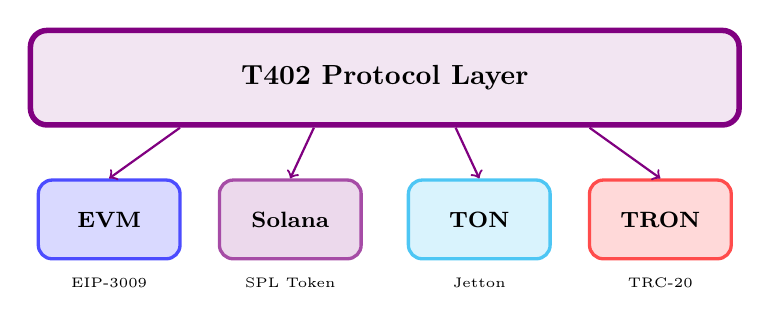
\begin{tikzpicture}[
    chainbox/.style={
        rectangle,
        rounded corners=5pt,
        minimum width=1.8cm,
        minimum height=1cm,
        line width=1.2pt,
        font=\bfseries\footnotesize
    },
    protocol/.style={
        rectangle,
        rounded corners=6pt,
        minimum width=9cm,
        minimum height=1.2cm,
        draw=violet,
        line width=2pt,
        fill=violet!10,
        font=\bfseries
    }
]

% Protocol layer
\node[protocol] (t402) at (0,1.8) {T402 Protocol Layer};

% Chains
\node[chainbox, draw=blue!70, fill=blue!15] (evm) at (-3.5,0) {EVM};
\node[chainbox, draw=violet!70, fill=violet!15] (sol) at (-1.2,0) {Solana};
\node[chainbox, draw=cyan!70, fill=cyan!15] (ton) at (1.2,0) {TON};
\node[chainbox, draw=red!70, fill=red!15] (tron) at (3.5,0) {TRON};

% Features
\node[font=\tiny] at (-3.5,-0.8) {EIP-3009};
\node[font=\tiny] at (-1.2,-0.8) {SPL Token};
\node[font=\tiny] at (1.2,-0.8) {Jetton};
\node[font=\tiny] at (3.5,-0.8) {TRC-20};

% Connections
\draw[->, thick, violet] (t402.south) ++(-2.6,0) -- (evm.north);
\draw[->, thick, violet] (t402.south) ++(-0.9,0) -- (sol.north);
\draw[->, thick, violet] (t402.south) ++(0.9,0) -- (ton.north);
\draw[->, thick, violet] (t402.south) ++(2.6,0) -- (tron.north);

\end{tikzpicture}
\caption{T402 multi-chain architecture with unified protocol layer}
\label{fig:multichain}
\end{figure}

Each blockchain network is identified using CAIP-2 format (e.g., \code{eip155:8453} for Base), enabling:

\begin{itemize}
    \item Unambiguous network identification
    \item Support for multiple networks per blockchain family
    \item Future extensibility to new networks
\end{itemize}

\section{Protocol Versioning}
\label{sec:versioning}

\tprotocol{} uses the \code{t402Version} field for protocol versioning:

\begin{table}[h]
\centering
\caption{Protocol Version History}
\label{tab:versions}
\begin{tabular}{clp{7cm}}
\toprule
\textbf{Version} & \textbf{Date} & \textbf{Changes} \\
\midrule
1 & 2025-08 & Initial release with legacy network identifiers \\
2 & 2025-12 & CAIP-2 networks, \code{resource} separation, extensions support \\
\bottomrule
\end{tabular}
\end{table}

\begin{warningbox}[Version 1 Deprecation]
Protocol version 1 is deprecated and no longer receives security updates. All implementations should migrate to version 2. See Appendix for migration guidance.
\end{warningbox}
